\documentclass[a4paper,12pt]{article}

\usepackage[a4paper, inner=1.7cm, outer=2.7cm, top=1.5cm, bottom=2cm, bindingoffset=1.2cm]{geometry}
\usepackage[german]{babel}
\usepackage{microtype}
\usepackage{fancyhdr}
\usepackage{hyperref}
\usepackage[pdftex]{graphicx}

\pagestyle{fancy}
\fancyfoot[C]{\thepage}

\newcommand{\myparagraph}[1]{\paragraph*{#1}\mbox{}\\}

\title{Dokumentation zur Projektaufgabe für das Modul Tool- und Pluginprogrammierung im Sommersemester 2022} 
\author{Oliver Jakobs}

\begin{document}

\maketitle

\section*{Thema und Motivation}

Als Thema für meine Modulaufgabe habe ich mich für \textbf{Entwicklung einer Mesh Decimation-Anwendung} entischieden, da ich in meinem nächsten privaten Projekt mit 3D-Meshes arbeiten will und ich dann potenziell Verwendung für einen Mesh Decimation Algorithmus finde.

Da mir der Low-Poly Style gefällt und ich diesen auch in meinen privaten Projekten verwenden will, kann ich durch eine Mesh Decimation-Anwendung alle Modelle auf einen passenden Face-Count reduzieren.

Außerdem kann ich mit dem Algorithmus mehrerer Versionen mit unterschiedlichen \emph{Level-of-detail} erstellen, was das Rendern für Videospiele effizienter machen kann.
\\
\\
Während meiner Recherche bin ich auf ein Paper mit dem Titel '\emph{Surface Simplification Using Quadric Error Metrics}' von Michael Garland und Paul S. Heckbert gestoßen und habe mich dafür entschieden den in diesem Paper vorgestellten Algorithmus (zumindestens teilweise) zu implementieren. 
Dieses Paper habe ich auch meiner Abgabe beigefügt.

Da in dem Paper von Mesh oder Surface Simplification anstelle von Mesh Decimation gesprochen wird, werde ich das Verfahren auch Simplification nennen. 
\\
\\
Da ich am Anfang bisschen überfordert war und nicht wirklich wusste wo ich anfangen soll, habe ich nach anderen Implementionen gesucht, durch die ich den Algorithmus besser verstehen kann. Dabei habe ich ein GitHub Repository (\url{https://github.com/Meirshomron/MeshSimplification}) gefunden, das mir vor allem bei der Umsetzenung der Fehlerberechnung geholfen hat.

\newpage

\section*{Designentscheidungen}

Meine Designentscheidungen unterteile ich in zwei Abschnitte. Im ersten Abschnitt geht es um allgemeine Entscheidungen, bei denen es um den Umfang des Projektes oder die Benutzerschnittstelle geht. Im zweiten Abschnitt geht es dann um Entscheidungen, die die eigentliche Implementation des Algorithmus betreffen.

\subsection*{Allgemeine Entscheidungen}

\myparagraph{Umfang des Projektes}
Das Programm soll ein 3D-Model mit dem Format \texttt{.obj} laden und anzeigen können. Dann soll über ein GUI ausgewählt werden können auf wie viele Faces das Mesh reduziert werden soll. Durch einen Button soll dann der Algorithmus mit den vorher festegelegtem Ziel ausgeführt werden. Außerdem soll es einen Button geben, der das Mesh auf seinen ursprünglichen Zustand zurücksetzt.
\\
\\
Des Weiteren habe ich mich gegen den Export in ein Dateiformat entschieden, da es von der Komlexität eher trivial ist und ich im Normalfall in ein Engine-Spezifisches Format exportieren würde.

\myparagraph{Rendering}
Für das Renderering habe ich für Flat-Shading entschieden. Dadurch werden die Faces eines Meshes hervorgehoben und die Veränderungen durch die Mesh-Simplification werden offensichtlicher.
Außerdem können die für das Flat-Shading benötigten Face-Normals im Fragment-Shader berechnet werden, wodurch es möglich ist, dass die Vertices, was das Rendern betrifft, nur aus Positionen bestehen. 

\myparagraph{Ein- und Ausgabe des Algorithmus}
Wenn ein Vertex also einfach nur ein \texttt{vec3} ist, wird das Laden des Meshes einfacher (und schneller) und ich habe für die Eingabe in den Simplification-Algorithmus einen Vektor für die Vertices (also die Positionen) und einen Vektor für die Indices, die die Faces bilden. Diese beiden Vektoren gibt der Algorithmus dann auch wieder (verändert) aus.

\subsection*{Entscheidungen zur Algorithmus Implementation}

\myparagraph{Darstellung der Vertices}
Für den von mir gewählten Algorithmus muss einem Vertex eine Position und eine Fehler-Matrix zugeordnet werden können.
Das realisiere ich durch zwei Vektoren (einen für die Positionen und einen für die Fehler-Matrizen), indem ich den Vertex durch einen Index darstelle.

Um jetzt an die Position eines Vertex \emph{v} zu gelangen, muss nur der \emph{v}-te Eintrag aus dem Vektor der Positionen ausgelesen werden. Für die Fehler-Matrix eines Vertex funktioniert das analog.

Der Grund warum ich mich für diese Darstellung der Daten entschieden hab ist, weil ich dadruch den geringsten Aufwand bei der Ein- und Ausgabe in bzw. aus dem Algorithmus habe. 
Ich will nicht die Positionen in Vertices mit Fehler-Matrizen umrechnen, oder die Fehler-Matrizen außerhalb des Algorithmus mit rumschleppen müssen.

\myparagraph{Ablauf des Algorithmus}
In dem Paper wird der Algorithmus in die folgenden fünf Schritte zusammengefasst:

\begin{enumerate}
	\item Berechne die Fehlermatrizen für alle Vertices.
	\item Auswahl aller möglichen Paare.
	\item Berechne für jedes Paar die neue Position des Vertex, wenn dass Paar zusammen gefasst wird.
	\item Plaziere die Paare in einem Heap, wobei die Sortierung anhand der Kosten der Paare erfolgt.
	\item Entferne wiederholt ein Paar mit geringsten Kosten, fasse das Paar zu einen neuen Vertex zusammen und passe alle Faces und Paare an.
\end{enumerate}

Schritte eins bis vier erfolgen in der Funktion \texttt{setup(vertices, indices)} (diese Funktion wird auch im Contructor der \texttt{MeshSimplifier} Klasse aufgerufen).

Schritt fünf wird in der Funktion \texttt{run(targetFaces)} in einer Schleife solange ausgeführt bis die angegebene Anzahl an Faces erreicht ist.

\myparagraph{Erstellen der Vertex Paare}
Bei dem Berechnen aller möglichen Paare ist es in dem Paper nicht notwendig, dass zwischen den beiden Verices eines Paares auch eine Kante existiert, solange die Distanz zwischen den Vertices einen festgelegten Threshold nicht überschreitet. 
Dadurch ist der Algorithmus vielseitiger anwendbar.
Für meine Implementation habe ich mich aber dafür entschieden diesen Threshold auf Null zu setzen und dadurch nur Paare zuzulassen, zwischen dessen Vertices auch eine Kante existiert, da so der Umfang von meinem Projekt überschaubarer bleibt.
\\
\\
Um beim Erstellen dieser Paare Duplikate zu verhindern, verwende ich ein temporäres \texttt{std::unordered\textunderscore set}.
Dabei sind zwei Paare $a$ und $b$ identisch, wenn:
$$(a.first=b.first \land a.second=b.second) \lor (a.second=b.first \land a.first=b.second)$$

Nachdem das Set gefüllt wurde, wandle ich es in einen \texttt{std::vector} um.
Das ist meiner Meinung nach die eleganteste Möglichkeit einen Vektor zu erstellen, in dem es keine Duplikate gibt (vorausgesetzt es werden alle Elemente aufeinmal hinzugefügt).

\myparagraph{Auswahl des nächsten Paares}
Wie vorher schon erwähnt werden die Paare (mit \texttt{std::make\textunderscore heap}) in einem Min Heap verwaltet. 
Dadurch ist es möglich mit \texttt{std::pop\textunderscore heap} ein günstigstes Paar zu entfernen und zu einem neuen Vertex zusammen zu fassen. 

\myparagraph{Veränderung der Vertices}
Für jedes Paar, das vereint wird, wird einer der beiden Vertices verändert.
Für den anderen Vertex werden lediglich die Faces und Paare, von denen er ein Teil ist angepasst.
Der eigentliche Vertex wird aber nicht entfernt, es gibt nur keinen Index mehr der auf ihn verweist.
Das wirkliche entfernen der überflüssigen Vertices würde ich erst beim exportieren durchführen.

\newpage
\section*{Bedienung}

Um das Programm zu starten muss die Datei \texttt{MeshSimplifier.exe} ausgeführt werden. Dafür wird neben der \texttt{.exe} auch der gesammte Inhalt des Orderns \texttt{./res/} benötigt.
\\
\\
Im ersten Abschnitt des GUIs (A) werden die Anzahl der Vertices und der Faces angezeigt (Da in meiner Implementation nicht mehr benötigte Vertices nicht entfernt werden, wird sich die Anzahl der Vertices bei einer Vereinfachung des Meshes nicht verändern).

Außerdem können hier die verfügbaren Meshes ausgewählt und geladen werden (B). Zu Verfügung stehen ein einfacher Würfel (8 Vertices, 12 Faces), ein Affenkopf (2012 Vertices, 3936 Faces) und die Marsienne Base (13235 Vertices, 27894 Faces) aus Übung03.
\\
\\
Der zweite Abschnitt (C) ist die Bedienung des Simplifiers. Hier kann mit einem Slider die gewünschte Anzahl an Faces ausgewählt werden (der Slider geht von 0 bis zur Anzahl der Faces der aktuellen Version des Meshes). Mit dem Button \texttt{Simplify} wird das Mesh so lange vereinfacht, bis die gewünschte Anzahl an Faces erreicht wurde. Mit dem Button \texttt{Reset} wird die ursprüngliche Version des Meshes wieder hergestellt.
\\
\\
Im letzten Abschnitt (D) befinden sich zwei Render-Optionen mit denen der Wireframe-Modus ein- und ausgeschaltet bzw. das Backface Culling aktiviert und deaktiviert werden kann.

\begin{figure}[h]
	\centering
	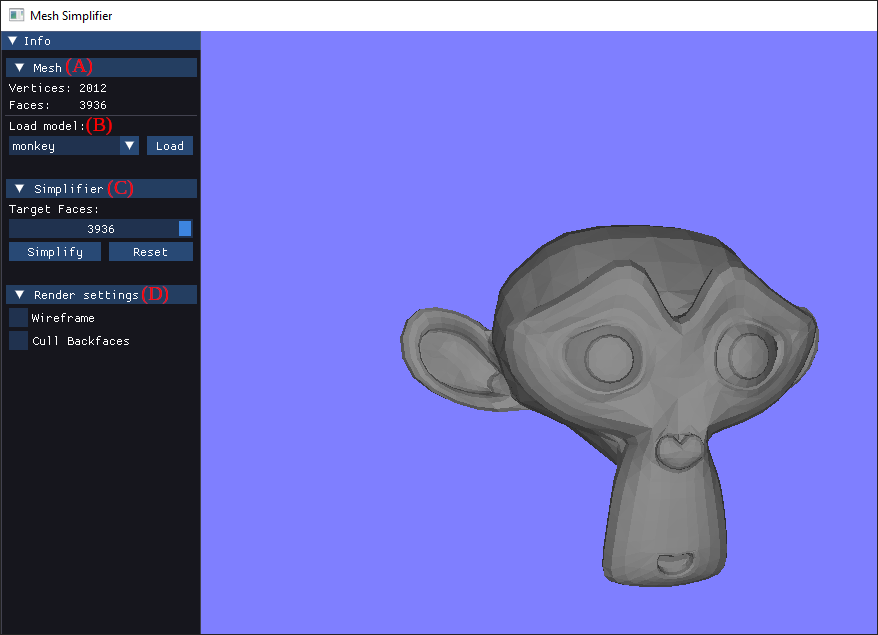
\includegraphics[width=\linewidth]{gui.png}
\end{figure}

Im Hauptbereich der Anwenung wird die aktuelle Version des Meshes gerendert. Mit Hilfe der linken Maustaste kann die Kamera auf einem Arcball um das Mesh bewegt werden.
\\
\\
Mit \texttt{Esc} kann das Programm beendet werden.

\section*{Bibliotheken}

In diesem Projekt verwende ich vier bzw. fünf Bibliotheken, die es mir ermöglichen eine grafischen Anwendung zu entwickeln, in der der Algorithmus an einem Modell ausgeführt werden kann.

\begin{itemize}
	\item \textbf{GLFW (\url{https://www.glfw.org/}):}
	GLFW ist eine Bibliothek, die es ermöglicht ein Fenster mit OpenGL-Kontext zu erstellen. 
	Außerdem wird durch diese Bibliothek die Eingabe mit Maus und Tastatur ermöglicht.
	Ich habe mich dafür entschieden, da ich damit die meiste Erfahrung habe und gut damit klar komme.
	\item \textbf{Ignis (\url{https://github.com/oliverjakobs/Ignis}):}
	Ignis ist ein von mir selbst entwickeltes Framework, das mir für meine Projekte den Umgang mit OpenGL vereinfachen soll. 
	Mit Ignis kann ich mit wenig Aufwand OpenGL-Objekte wie Shader oder Vertex-Arrays erstellen.
	\item \textbf{GLAD (\url{https://glad.dav1d.de/}):} 
	Glad ist eine OpenGL-Loading-Library und ist in Ignis integriert.
	\item \textbf{Dear ImGui (\url{https://github.com/ocornut/imgui}):}
	Dear ImGui ist eine eine Bibliothek zum Erstellen von Grafischen Benutzeroberflächen basierend auf dem \emph{Immediate Mode GUI} Paradigma.
	Durch Dear ImGui kann ich meiner Anwendung eine grafische Benutzeroberfläche geben, und somit die Bedienung vereinfachen.
	\item \textbf{glm (\url{https://github.com/g-truc/glm}):}
	Glm ist eine Mathe-Bibliothek basierend auf den \emph{OpenGL Shading Language (GLSL) Spezifikationen}. 
	Ich benutze glm, damit ich mir keine Gedanken machen muss, ob alle mathematischen Operationen auch wirklich richtig funktionieren. 
\end{itemize}

\section*{Build}

Zur Project Generation benutze ich Premake (\url{https://premake.github.io/}). Ich habe die entsprechenden Scripts meiner Abgabe beigefügt.
Falls also Probleme mit der VisualStudio Solution autreten sollten,
kann mit dem folgenden Befehl das Projekt neu generiert werden und so die Probleme hoffentlich gelöst werden:
\[\texttt{.\textbackslash premake\textbackslash premake5.exe [action]}\]
Für mein Projekt habe ich \texttt{vs2019} als \texttt{action} verwendet. Andere Möglichkeiten sind hier \url{https://premake.github.io/docs/Using-Premake} aufgelistet.


\end{document}